\section{Aufbau}
\label{sec:Aufbau}

In Abbildung \ref{fig:Aufbau} ist der experimentelle Aufbau des Versuchs zu sehen.
Der verwendete Halbleiter GaAs ist durchlässig für infrarotes Licht.
Als Lichtquelle wird deshalb eine Halogenlampe verwendet.
Nach der Bündelung des Lichtes über eine Sammellinse, wird es über ein sich drehendes Rad, den Lichtzerhacker, in Lichtpulse aufgeteilt.
Der Polarisator teilt den Lichtstrahl durch unterschiedliche Brechungsindizes der Komponenten im Polarisatormedium in einen ordentlichen s- und einen außerordentlich p-polarisierten Teil. Der s-Anteil wird dabei total reflektiert, während der p-Anteil transmittiert wird.
Das nun linear polarisierte Licht fällt auf eine Probe aus Galliumarsenid, welche sich im Feld eines Elektromagneten befindet. Über einen Interferenzfilter wird eine bestimmte Wellenlänge herausgefiltert und der Lichtstrahl trifft auf einen weiteren als Analysator dienenden Polarisator. Aus diesem treten zwei zueinander orthogonal polarisierte Strahlen aus, welche an zwei Photowiderstände Spannungen erzeugen.
Diese werden in einen Differenzverstärker gegeben, der an ein Oszilloskop angeschlossen ist. Die Frequenz des Differenzverstärkers ist zur Rauschunterdrückung auf die des Lichzerhackers abgestimmt und die ausgehende Spannung ist genau dann $0$, wenn die beiden vermessenen identisch sind.

\begin{figure}
\centering
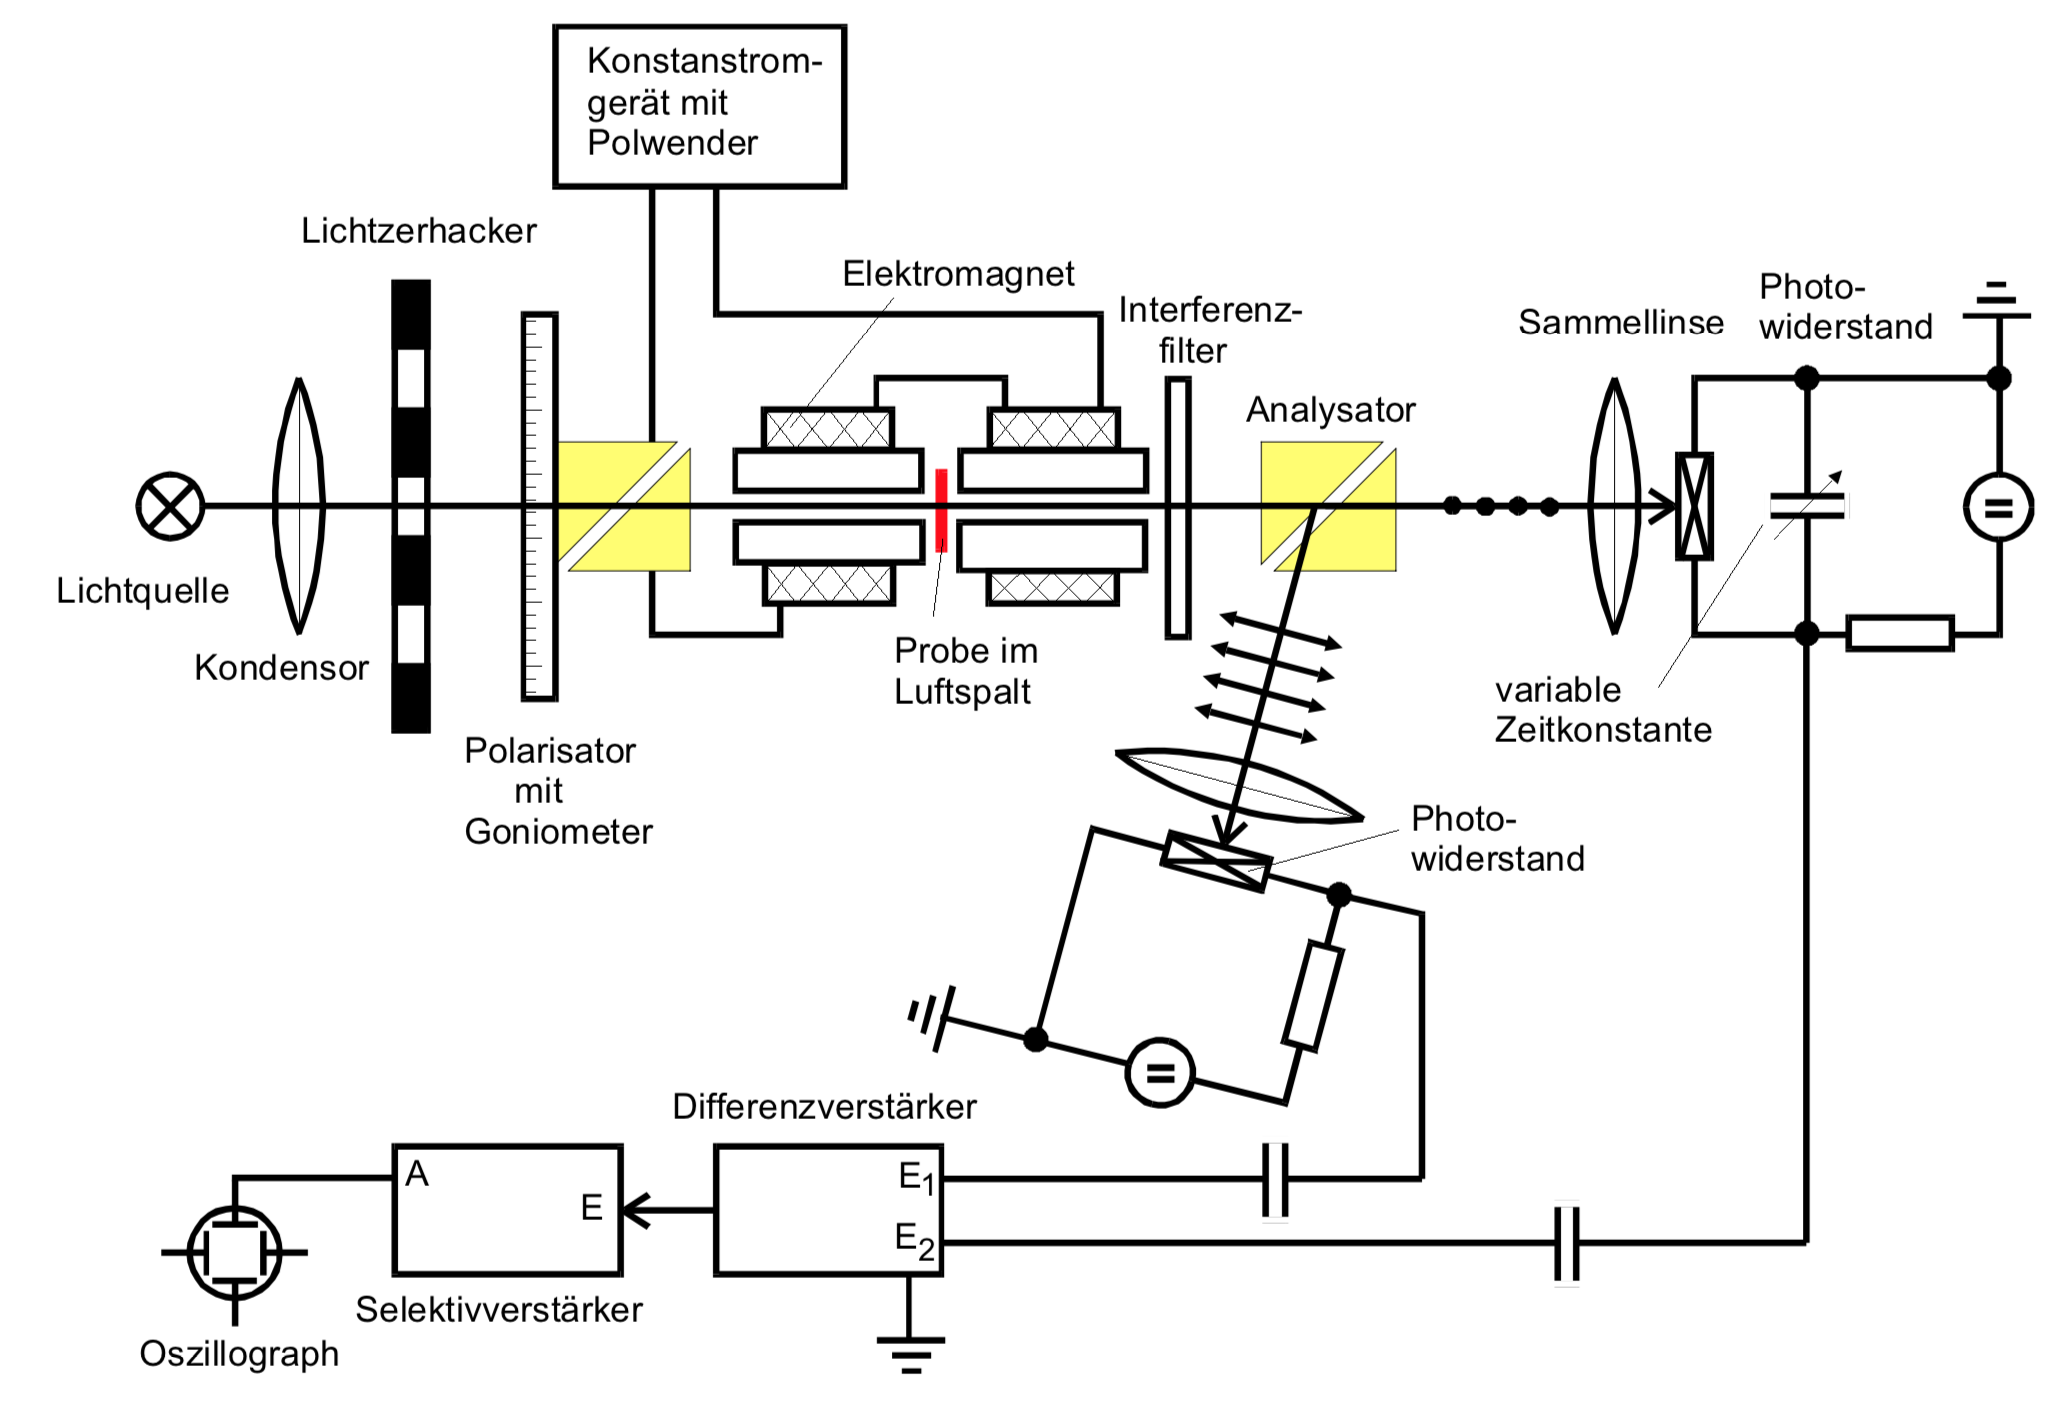
\includegraphics[width=0.9\textwidth]{content/images/aufbau.png}
\caption{Schematischer Aufbau zur Untersuchung der Faraday-Rotation.\cite{V46}}
\label{fig:Aufbau}
\end{figure}